\RequirePackage{pdf14}
\pdfminorversion=5
\pdfobjcompresslevel=1
\pdfcompresslevel=9

% define document class and font size
\documentclass[a4paper,oneside,12pt]{report}

% imports
\usepackage[utf8]{inputenc}
\usepackage[square, numbers, comma, sort&compress]{natbib}
\usepackage[top=2.50cm, bottom=2.50cm, left=3.00cm, right=3.00cm, includefoot]{geometry}
\usepackage[english,estonian]{babel}
\usepackage[printonlyused]{acronym}
\usepackage{amssymb} % http://ctan.org/pkg/amssymb
\usepackage{pifont}  % http://ctan.org/pkg/pifont
\usepackage{authoraftertitle}
\usepackage{nameref}
\usepackage{color}
\usepackage{caption}
\usepackage{graphicx}
\usepackage{indentfirst}
\usepackage{listings}
\usepackage[svgnames]{xcolor}
\usepackage{textcomp}
\usepackage{lmodern}
\usepackage{setspace}
\usepackage{tablefootnote}
\usepackage{multicol}
\usepackage{tikz}
\usepackage{times}
\usepackage{booktabs}
\usepackage{titlesec}
\usepackage{verbatim}
\usepackage[hyphens]{url}
\usepackage[hidelinks]{hyperref}
\usepackage[all]{hypcap}
\usepackage[T1]{fontenc}
\usepackage{lastpage}
\usepackage[figure,table,xspace]{totalcount}

% set title, author and date values. Check chapters/declaration.tex for name
\title{Insert title here}
\author{Anti Räis}
\date{2015}

% Generate PDF metadata - show PDF metadata with $ make info
\makeatletter
\hypersetup{
    pdfauthor   = {\@author},
    pdftitle    = {\@title},
    pdfsubject  = {TUT, master's thesis},
    pdfkeywords = {keyword_a, keyword_b},
%    pdfproducer = {},
%    pdfcreator  = {},
}
\makeatother

% define colors for syntax highlight text highlight
\definecolor{marktext}      {HTML}{000000}
\definecolor{markback}      {HTML}{FFFF00}
\definecolor{codegreen}     {HTML}{A6E22E}
\definecolor{codegray}      {HTML}{808080}
\definecolor{codestring}    {HTML}{880000}
\definecolor{backcolor}     {HTML}{FFFFFF}
\definecolor{maroon}        {rgb}{0.5,0,0}
\definecolor{darkgreen}     {rgb}{0,0.5,0}

\newcommand{\hl}[1]{\fboxsep0pt\colorbox{markback}{\color{marktext}\bfseries#1}}
\newcommand{\apos}{\textquotesingle}
\newcommand{\cmark}{\ding{51}}
\newcommand{\xmark}{\ding{55}}
\newcommand*{\fullref}[1]{\hyperref[{#1}]{\ref*{#1} ``\nameref*{#1}''}}

% configure listing
\lstdefinestyle{base}{
    aboveskip           = 2.0em,
    backgroundcolor     = \color{backcolor},
    basicstyle          = \footnotesize\ttfamily\mdseries,
    belowskip           = 0.0em,
    breakatwhitespace   = false,
    breaklines          = true,
    caption             = \lstname,
    captionpos          = b,
    commentstyle        = \color{gray}\ttfamily,
    extendedchars       = true,
    frame               = tb,
    keepspaces          = true,
    keywordstyle        = \color{blue},
    language            = html,
    morecomment         = [l][basicstyle]{http://},
    morecomment         = [l][basicstyle]{https://},
    numbers             = left,
    numbersep           = 5pt,
    numberstyle         = \color{codegray},
    showspaces          = false,
    showstringspaces    = false,
    showtabs            = false,
    stringstyle         = \color{codestring},
    tabsize             = 2,
    upquote             = true,
}
\lstset{style=base, columns=flexible, literate=
  {ä}{{\"a}}1 {ë}{{\"e}}1 {ï}{{\"i}}1 {ö}{{\"o}}1 {ü}{{\"u}}1
  {Ä}{{\"A}}1 {Ë}{{\"E}}1 {Ï}{{\"I}}1 {Ö}{{\"O}}1 {Ü}{{\"U}}1
  {â}{{\^a}}1 {ê}{{\^e}}1 {î}{{\^i}}1 {ô}{{\^o}}1 {û}{{\^u}}1
  {Â}{{\^A}}1 {Ê}{{\^E}}1 {Î}{{\^I}}1 {Ô}{{\^O}}1 {Û}{{\^U}}1
  {€}{{\EUR}}1 {£}{{\pounds}}1        {Õ}{{\~O}}1 {õ}{{\~o}}1
}

% configure XML syntax highlight
\lstdefinelanguage{XML}
{
    morestring      = [s]{"}{"},
    morecomment     = [s]{?}{?},
    morecomment     = [s]{!--}{--},
    commentstyle    = \color{darkgreen},
    moredelim       = [s][\color{black}]{>}{<},
    moredelim       = [s][\color{red}]{\ }{=},
    stringstyle     = \color{blue},
    identifierstyle = \color{maroon},
}

% configure JavaScript syntax highlight
\lstdefinelanguage{JavaScript}{
    keywords        = {break, case, catch, continue, debugger, default, delete, do, else, false, finally, for, function, if, in, instanceof, new, null, return, switch, this, throw, true, try, typeof, var, void, while, with},
    morecomment     = [l]{//},
    morecomment     = [s]{/*}{*/},
    morestring      = [b]',
    morestring      = [b]",
    ndkeywords      = {class, export, boolean, throw, implements, import, this},
    keywordstyle    = \color{blue}\bfseries,
    ndkeywordstyle  = \color{darkgray}\bfseries,
    identifierstyle = \color{black},
    commentstyle    = \color{codegray}\ttfamily,
    stringstyle     = \color{red}\ttfamily,
    sensitive       = true
}

% Configure titles
\titleformat{\chapter}{}{\bf\LARGE\thechapter.~}{1em}{\bf\LARGE}
%\titlelabel{\thetitle.\quad}
%\captionsetup{labelsep=period}

% Configure graphics folder
\graphicspath{{img/}}

\renewcommand{\bibname}{References}
\renewcommand\lstlistingname{Code example}
\renewcommand\lstlistlistingname{Code examples}

\onehalfspacing
\setlength{\parindent}{2em} % Indent all paragraphs
\setlength{\parskip}{1em}

% document styling and configuration
\begin{document}
% For debuggin overlong lines!
% \overfullrule = 2cm

% So that \url{} would break and stuff wouldn't "run over the edge"
\sloppy

% Fix footnotes splitting in multiple pages
\interfootnotelinepenalty=10000

\begin{titlepage}
\begingroup
    \singlespace
    \begin{center}
            TALLINN UNIVERSITY OF TECHNOLOGY \\
            Faculty of Information Technology \\
            Department of Computer Science \\
            TUT Centre for Digital Forensics and Cyber Security

        \vfill
            \huge \textbf{\MyTitle}\\[1cm]
            \large Master's thesis\\[1cm]
            <INSERT THESIS CODE HERE>\\[4cm]
            \normalsize

            \begin{flushright}
                \MyAuthor \\
                STUDENT CODE\\[1.5cm]
                Supervisors \\
                Supervisor A, MSc\\
                Supervisor B, PhD\\
            \end{flushright}
        \vfill

        Tallinn \MyDate
    \end{center}
\endgroup
\end{titlepage}

\pagenumbering{roman}
\chapter*{Declaration}
\label{declaration}
\thispagestyle{empty}
\selectlanguage{english}

\vspace{30mm}
I declare that this thesis is the result of my own research except as cited in the references.
The thesis has not been accepted for any degree and is not concurrently submitted in candidature
of any other degree.
\vspace{30mm}

\begin{minipage}{0.50\textwidth}
    \begin{flushleft}\today\end{flushleft}
\end{minipage}
\begin{minipage}{0.44\textwidth}
    \begin{flushright}
    Anti Räis \\
    \vspace{0.5cm}
    ........................ \\
    (Signature)
    \end{flushright}
\end{minipage}

\newpage
\clearpage
\chapter*{Abstract}
\label{annotation}
\thispagestyle{empty}
Lorem ipsum dolor sit amet, consectetur adipiscing elit. Morbi sed dui a felis posuere porta. Curabitur congue euismod feugiat. Cum sociis natoque penatibus et magnis dis parturient montes, nascetur ridiculus mus. Etiam tempor pharetra ipsum non consequat. Phasellus tempor magna quam. Aliquam nunc diam, rhoncus et libero ultricies, euismod laoreet est. Mauris non pellentesque dui. Nunc elit sem, molestie eu nibh sed, cursus commodo felis. Etiam nec viverra dolor, vitae maximus nisl. Quisque eget orci et erat mollis feugiat. Cras dignissim, tortor finibus euismod euismod, mi diam gravida leo, ut sollicitudin diam dui id quam.

The thesis is in English and contains \pageref{LastPage} pages of text, 6 chapters, \totalfigures figures, \totaltables tables.


\clearpage
\chapter*{Annotatsioon}
\label{annotatsioon}
\thispagestyle{empty}
Lorem ipsum dolor sit amet, consectetur adipiscing elit. Morbi sed dui a felis posuere porta. Curabitur congue euismod feugiat. Cum sociis natoque penatibus et magnis dis parturient montes, nascetur ridiculus mus. Etiam tempor pharetra ipsum non consequat. Phasellus tempor magna quam. Aliquam nunc diam, rhoncus et libero ultricies, euismod laoreet est. Mauris non pellentesque dui. Nunc elit sem, molestie eu nibh sed, cursus commodo felis. Etiam nec viverra dolor, vitae maximus nisl. Quisque eget orci et erat mollis feugiat. Cras dignissim, tortor finibus euismod euismod, mi diam gravida leo, ut sollicitudin diam dui id quam.

Lõputöö on kirjutatud Inglise keeles ning sisaldab teksti \pageref{LastPage} leheküljel, 6 peatükki, \totalfigures joonist, \totaltables tabelit.

\addtocounter{page}{1}


\singlespacing
\tableofcontents

\newpage
\onehalfspacing
\pagenumbering{arabic}

% include document content
\chapter{Introduction}
\label{introduction}

Lorem ipsum dolor sit amet, \texttt{consectetur} adipiscing elit. Morbi sed dui a felis posuere porta. Curabitur congue euismod feugiat. Cum sociis natoque penatibus et magnis dis parturient montes, nascetur ridiculus mus. Etiam tempor pharetra ipsum non consequat. Phasellus tempor magna quam. Aliquam nunc diam, rhoncus et libero ultricies, euismod laoreet est. Mauris non pellentesque dui. Nunc elit sem, molestie eu nibh sed, cursus commodo felis. Etiam nec viverra dolor, vitae maximus nisl. Quisque eget orci et erat mollis feugiat. Cras dignissim, tortor finibus euismod euismod, mi diam gravida leo, ut sollicitudin diam dui id quam.~\footnote{\url{http://www.example.com\#Examples}}

\ac{OWASP}
\acf{OWASP}
``Text''
``\texttt{\&}''
\texttt{"Literal quote: \textbackslash{}"; and single quote \apos "}
Text~``\texttt{\textasciitilde!*()'-.\_}''

He said something.~\cite{inproceedings}
He said something.~\cite{techreport}
He said something.~\cite{book}
He said something.~\cite{masterthesis}
He said something.~\cite{article}
He said something.~\cite{misc}
He said something.~\cite{online}

URL: \url{https://www.example.com?a=0&b=0}
Ref~\ref{appendix:a}

\section{Problem statement and contribution of the thesis}
Lorem ipsum dolor sit amet, consectetur adipiscing elit. Morbi sed dui a felis posuere porta. Curabitur congue euismod feugiat. Cum sociis natoque penatibus et magnis dis parturient montes, nascetur ridiculus mus. Etiam tempor pharetra ipsum non consequat. Phasellus tempor magna quam. Aliquam nunc diam, rhoncus et libero ultricies, euismod laoreet est. Mauris non pellentesque dui. Nunc elit sem, molestie eu nibh sed, cursus commodo felis. Etiam nec viverra dolor, vitae maximus nisl. Quisque eget orci et erat mollis feugiat. Cras dignissim, tortor finibus euismod euismod, mi diam gravida leo, ut sollicitudin diam dui id quam.

\begin{quote} % The goal should be as specific as possible
\emph{
    Lorem ipsum dolor sit amet, consectetur adipiscing elit. Morbi sed dui a felis posuere porta. Curabitur congue euismod feugiat. Cum sociis natoque penatibus et magnis dis parturient montes, nascetur ridiculus mus. Etiam tempor pharetra ipsum non consequat. Phasellus tempor magna quam. Aliquam nunc diam, rhoncus et libero ultricies, euismod laoreet est. Mauris non pellentesque dui. Nunc elit sem, molestie eu nibh sed, cursus commodo felis. Etiam nec viverra dolor, vitae maximus nisl. Quisque eget orci et erat mollis feugiat. Cras dignissim, tortor finibus euismod euismod, mi diam gravida leo, ut sollicitudin diam dui id quam.
}
\end{quote}

The expected outcome of this thesis is...
\begin{itemize}
    %\setlength\itemsep{0em}
    \item item a;
    \item item b;
    \item item c;
    \item item d.
\end{itemize}

\section{Some other section}
Lorem ipsum dolor sit amet, consectetur adipiscing elit. Curabitur eu velit eu erat tristique egestas a non leo. Maecenas et enim id lacus molestie ornare. Fusce ante ligula, accumsan sollicitudin sapien et, vulputate ultricies metus. Proin eget elementum turpis. Nulla cursus arcu in ex ultricies semper.

\begin{table}[h]
\centering
\footnotesize
\begin{tabular}{clcc}
    Entity & name    & decimal & hexadecimal \\
    \hline
    <      & \&lt;   & \&\#60; & \&\#x003C;  \\
    >      & \&gt;   & \&\#62; & \&\#x003E;  \\
    \&     & \&amp;  & \&\#38; & \&\#x0026;  \\
    '      & \&apos;
    ~\tablefootnote{Not supported by \ac{HTML}4 user-agents. Decimal encoding scheme should be used instead. Read \ac{W3C} recommendation: \url{http://www.w3.org/TR/xhtml1/\#C_16}}
                     & \&\#39; & \&\#x0027;  \\
    "      & \&quot; & \&\#34; & \&\#x0022;  \\
    \hline
\end{tabular}
\caption{HTML entity encoding}
\label{table:entity-encoding}
\end{table}

\section{Outline of the thesis}
Lorem ipsum dolor sit amet, consectetur adipiscing elit. Curabitur eu velit eu erat tristique egestas a non leo. Maecenas et enim id lacus molestie ornare. Fusce ante ligula, accumsan sollicitudin sapien et, vulputate ultricies metus. Proin eget elementum turpis. Nulla cursus arcu in ex ultricies semper.

\begin{figure}[h]
    \centering
    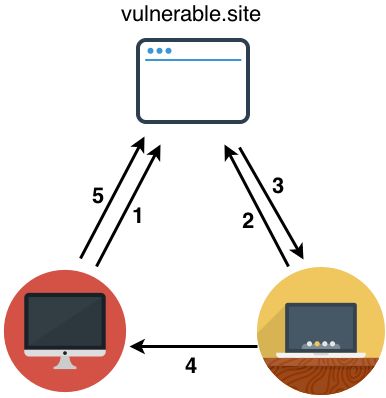
\includegraphics[keepaspectratio, width=0.5\textwidth]{image}
    \caption{Some image}
    \label{fig:image}
\end{figure}

\section{Ethical considerations}
Lorem ipsum dolor sit amet, consectetur adipiscing elit. Curabitur eu velit eu erat tristique egestas a non leo. Maecenas et enim id lacus molestie ornare. Fusce ante ligula, accumsan sollicitudin sapien et, vulputate ultricies metus. Proin eget elementum turpis. Nulla cursus arcu in ex ultricies semper.

\begin{lstlisting}[escapechar=|, caption=Example, label={example}]
Some HTML text
<h1 class="|\hl{red" onclick="alert(\apos XSS\&lt;\apos )}|">Title.</h1>
\end{lstlisting}

\section{Acknowledgments}
\label{acknowledgments}
Lorem ipsum dolor sit amet, consectetur adipiscing elit. Curabitur eu velit eu erat tristique egestas a non leo. Maecenas et enim id lacus molestie ornare. Fusce ante ligula, accumsan sollicitudin sapien et, vulputate ultricies metus. Proin eget elementum turpis. Nulla cursus arcu in ex ultricies semper.


\chapter{Second chapter}
\label{second-chapter}

\section{Sub-section}
Text.

\section{Sub-section}
Text.

\section{Section}
Text.

\subsection{Sub section}

\begin{enumerate}
    \item item a
    \item item b
    \item item c
\end{enumerate}

Text

\subsubsection{Sub-sub-section}
\label{label-1}

Text.




\chapter{Chapter 3}
\label{chapter-3-laber}

Text.

\section{Some Section}

Text.



\chapter{Conclusion}
\label{conclusion}

% What is the strongest and most important statement that you can make from your observations?
% If you met the reader at a meeting six months from now, what do you want them to remember about your paper?
% Refer back to problem posed, and describe the conclusions that you reached from carrying out this investigation, summarize new observations, new interpretations, and new insights that have resulted from the present work.
% Include the broader implications of your results.
% Do not repeat word for word the abstract, introduction or discussion.

The purpose ...

As a future development...

As a result...


\renewcommand \bibname{References}
\cleardoublepage
\phantomsection
\addcontentsline{toc}{chapter}{\bibname}
% \bibliographystyle{abbrvnat}
\bibliographystyle{unsrtnat}
\bibliography{references}

% Code examples
\cleardoublepage
\phantomsection
\addcontentsline{toc}{chapter}{\lstlistlistingname}
\lstlistoflistings

% List of Figures
\cleardoublepage
\phantomsection
\addcontentsline{toc}{chapter}{\listfigurename}
\listoffigures

% List of Tables
\cleardoublepage
\phantomsection
\addcontentsline{toc}{chapter}{\listtablename}
\listoftables

% List of acronyms
\cleardoublepage
\phantomsection
\addcontentsline{toc}{chapter}{}
\section*{List of Acronyms}
\begin{acronym}
    \acro{HTML}     {Hypertext Markup Language}
    \acro{OWASP}    {Open Web Application Security Project}
    \acro{W3C}      {World Wide Web Consortium}
    \acro{HIDDEN}   {``This is not referenced, therefore not seen in the list''}
\end{acronym}


\appendix
\chapter{Appendixes}

\section{Appendix A}
\label{appendix:a}

Some appendix text.

\newpage
\lstinputlisting[language=php, caption={PHP source code}, label={apx:chars-php}]{./code/php-example.php}




\end{document}
